\documentclass[10pt, a5paper]{article}
\usepackage{pdfpages}
\usepackage{parallel}
\usepackage[T2A]{fontenc}
\usepackage{ucs}
\usepackage[utf8x]{inputenc}
\usepackage[polish,english,russian]{babel}
\usepackage{hyperref}
\usepackage{rotating}
\usepackage[inner=2cm,top=1.8cm,outer=2cm,bottom=2.3cm,nohead]{geometry}
\usepackage{listings}
\usepackage{graphicx}
\usepackage{wrapfig}
\usepackage{longtable}
\usepackage{indentfirst}
\usepackage{array}
\newcolumntype{P}[1]{>{\raggedright\arraybackslash}p{#1}}
\frenchspacing
\usepackage{fixltx2e} %text sub- and superscripts
\usepackage{icomma} % коскі ў матэматычным рэжыме
\PreloadUnicodePage{4}

\newcommand{\longpage}{\enlargethispage{\baselineskip}}
\newcommand{\shortpage}{\enlargethispage{-\baselineskip}}

\def\switchlang#1{\expandafter\csname switchlang#1\endcsname}
\def\switchlangbe{
\let\saverefname=\refname%
\def\refname{Літаратура}%
\def\figurename{Іл.}%
}
\def\switchlangen{
\let\saverefname=\refname%
\def\refname{References}%
\def\figurename{Fig.}%
}
\def\switchlangru{
\let\saverefname=\refname%
\let\savefigurename=\figurename%
\def\refname{Литература}%
\def\figurename{Рис.}%
}

\hyphenation{admi-ni-stra-tive}
\hyphenation{ex-pe-ri-ence}
\hyphenation{fle-xi-bi-li-ty}
\hyphenation{Py-thon}
\hyphenation{ma-the-ma-ti-cal}
\hyphenation{re-ported}
\hyphenation{imp-le-menta-tions}
\hyphenation{pro-vides}
\hyphenation{en-gi-neering}
\hyphenation{com-pa-ti-bi-li-ty}
\hyphenation{im-pos-sible}
\hyphenation{desk-top}
\hyphenation{elec-tro-nic}
\hyphenation{com-pa-ny}
\hyphenation{de-ve-lop-ment}
\hyphenation{de-ve-loping}
\hyphenation{de-ve-lop}
\hyphenation{da-ta-ba-se}
\hyphenation{plat-forms}
\hyphenation{or-ga-ni-za-tion}
\hyphenation{pro-gramming}
\hyphenation{in-stru-ments}
\hyphenation{Li-nux}
\hyphenation{sour-ce}
\hyphenation{en-vi-ron-ment}
\hyphenation{Te-le-pathy}
\hyphenation{Li-nux-ov-ka}
\hyphenation{Open-BSD}
\hyphenation{Free-BSD}
\hyphenation{men-ti-on-ed}
\hyphenation{app-li-ca-tion}

\def\progref!#1!{\texttt{#1}}
\renewcommand{\arraystretch}{2} %Іначай формулы ў матрыцы зліпаюцца з лініямі
\usepackage{array}

\def\interview #1 (#2), #3, #4, #5\par{

\section[#1, #3, #4]{#1 -- #3, #4}
\def\qname{LVEE}
\def\aname{#1}
\def\q ##1\par{{\noindent \bf \qname: ##1 }\par}
\def\a{{\noindent \bf \aname: } \def\qname{L}\def\aname{#2}}
}

\def\interview* #1 (#2), #3, #4, #5\par{

\section*{#1\\{\small\rm #3, #4. #5}}

\def\qname{LVEE}
\def\aname{#1}
\def\q ##1\par{{\noindent \bf \qname: ##1 }\par}
\def\a{{\noindent \bf \aname: } \def\qname{L}\def\aname{#2}}
}

\begin{document}
\title{Разглядывая атомы. Программное обеспечение для визуализации химического строения вещества\footnote{\url{tenebrosus.scriptor@gmail.com}, \url{http://lvee.org/ru/abstracts/218}}}
\author{Антон Літвіненка, Kyiv, Ukraine}
\maketitle
\begin{abstract}
Brief review of main types and uses of software for chemical structures visualization is presented in this abstract. Current situation with free chemical visualization software as well as some actual tasks and problems in chemical structure analysis are discussed.
\end{abstract}
Одни из важнейших объектов, которыми оперирует химия, "--- атомы и молекулы "--- практически недоступны для прямого экспериментального наблюдения. В то же время, взаимное расположение атомов в веществе несет важнейшую информацию о его строении и возможных свойствах. В настоящее время для анализа строения вещества на атомно-молекулярном уровне активно применяется специализированное программное обеспечение.

Целью работы является обзор существующих типов графического представления атомно-молекулярной структуры вещества, основных задач (решенных и актуальных) такого представления, и ситуации со свободным программным обеспечением для визуализации химических структур.

С помощью ПО для визуализации химических структур решаются следующие задачи:

\begin{itemize}
  \item Подготовка рисунков для публикаций;
  \item Анализ параметров структуры (измерение расстояний между атомами, углов между связями, проверка наличия пустот и т.д.);
  \item Подготовка входных данных для других программ, выполняющих анализ или моделирование (квантовохимическое, \linebreak молекулярно-механическое, поиск по базам данных и т.д.)
  \item Анализ результатов вычислений, выполненных другими программами.
\end{itemize}

Большинство программ для визуализации предоставляет также широкие возможности для редактирования химических структур или создания их с нуля.

Основными элементами для отображения являются \textbf{атом} и \linebreak\textbf{связь}.

\subsubsection*{2D и <<2,5D>> визуализаторы (редакторы).}

Отображают исключительно связность атомов в \linebreak химической структуре (как правило, органической молекуле), не отображая расположения атомов в пространстве друг относительно друга, а также длин связей, углов между связями и расстояний между атомами (рис. ~\ref{Litvenenka1}). Атомы обозначаются символами соответствующих элементов или вершинами геометрических фигур (вершина без символа обозначает атом углерода); атомы водорода, как правило, опускаются (они могут быть достроены в воображении зрителя, исходя из валентностей атомов, около которых находятся). Связи обозначаются ребрами геометрических фигур (стиль отрисовки линии обозначает тип связи "--- одинарная, двойная, тройная, координационная и т.д.). Кроме единичных формул, могут изображаться схемы реакций. Изображение плоское (2D) и, как правило, не требует цвета и сложных полутонов "--- таким образом, рисунки такого типа могут быть без адаптации использованы для печатных работ. В подавляющем большинстве случаев структуры сохраняются в специальных форматах, рисунок может быть экспортирован в виде растрового или векторного графического файла, а также (под Windows) с помощью OLE. Подписи, стрелки и другие элементы схем могут быть добавлены как в самом редакторе, так и при постобработке.


\begin{figure}[h!]
  \centering
  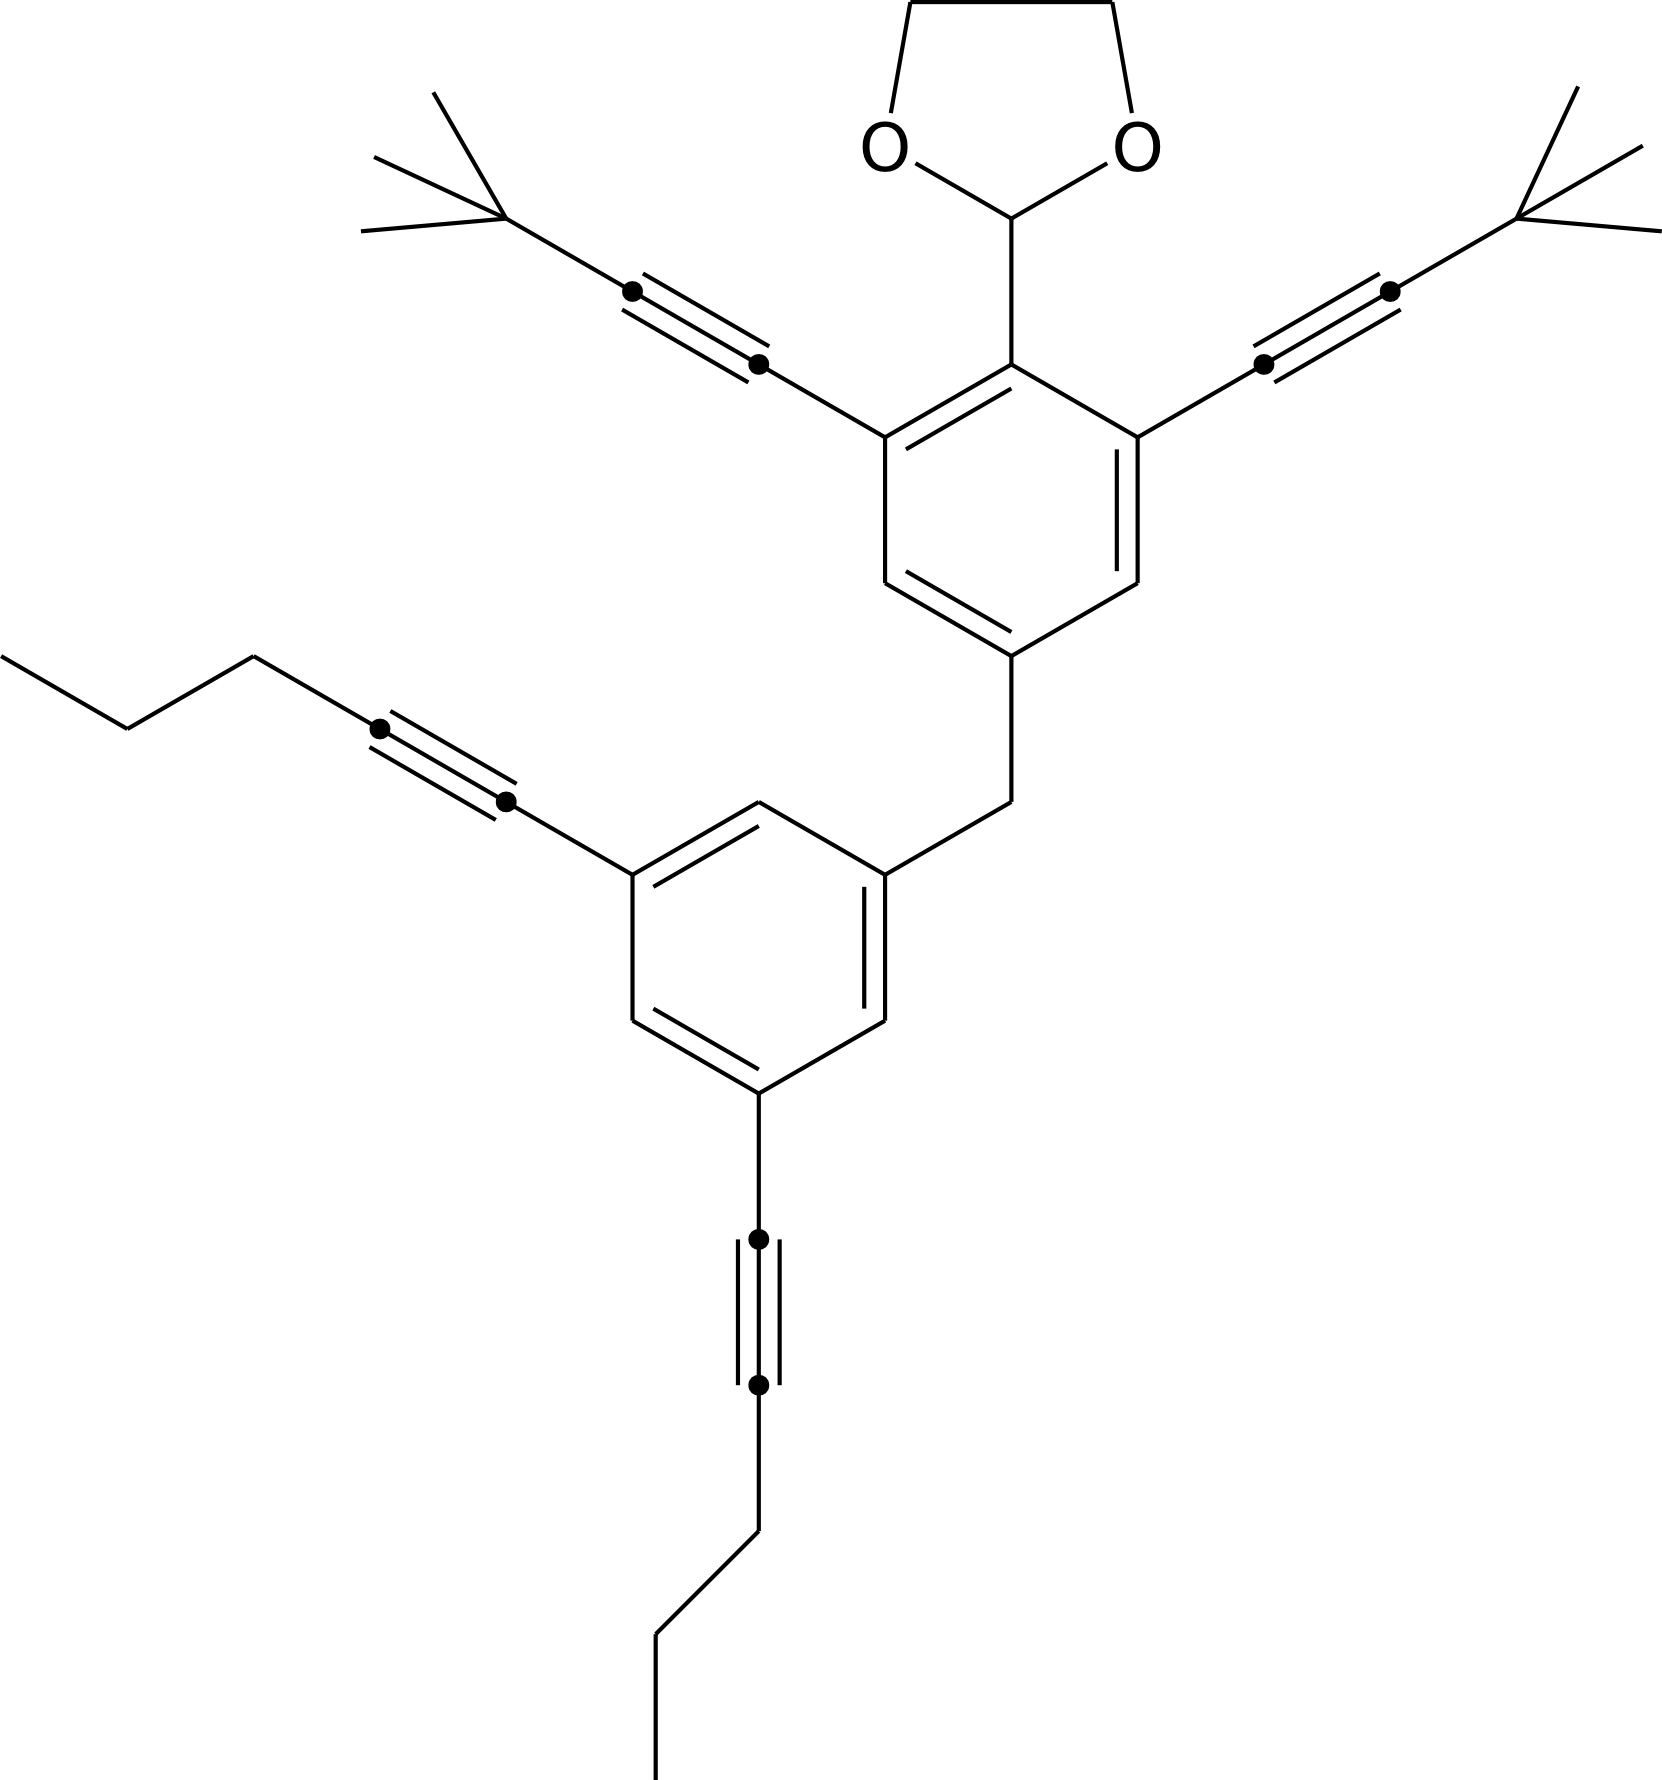
\includegraphics[width=5cm]{20_2016_Litvenenka1.png}
  \caption{Пример органической молекулы, нарисованный в GChemPaint (перерисовано автором по формуле, приведенной в работе ~\cite{Litvenenka1}).}
  \label{Litvenenka1}
\end{figure}

Исторически подобный способ изображения молекул (несколько отличающийся по используемым обозначениям) появился в середине XIX века ~\cite{Litvenenka2}. Для нужд современной органической химии были добавлены условные обозначения и стандартные проекции, необходимые для указания конфигурации оптических изомеров (рис. ~\ref{Litvenenka2}) "--- таким образом, этот способ изображения молекул является чем-то средним между 2D и 3D.

\begin{figure}[h!]
  \centering
  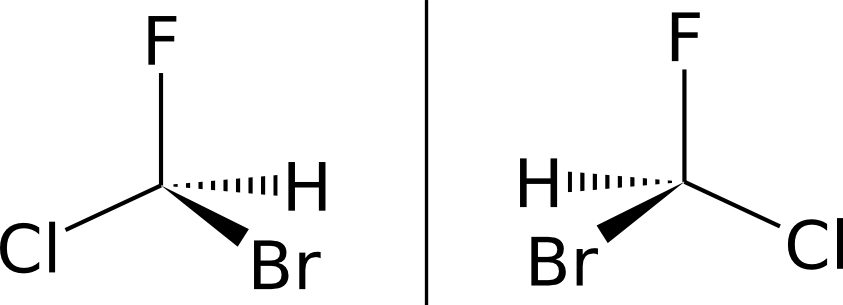
\includegraphics[width=5cm]{20_2016_Litvenenka2.png}
  \caption{Два оптических изомера бромфторхлорметана, отличающиющиеся только ориентацией заместителей. Связь, обозначенная сплошным треугольником, обозначает атом, находящийся перед плоскостью рисунка, штрихованым "--- за плоскостью рисунка.}
  \label{Litvenenka2}
\end{figure}

Дополнительное использование "--- подготовка запросов для поиска по базам данных (по фрагменту структуры), а также для предсказания ЯМР-спектров.

Свободное ПО для 2D-визуализации (GChemPaint, BKChem) существует, однако имеет очень бедный функционал и проигрывает в сравнении с проприетарными аналогами (ACD/ChemSketch, ISIS/Draw). Шаблоны для LaTeX еще беднее по возможностям и используются крайне редко.

\subsubsection*{3D визуализаторы}

Изображают координаты атомов в трехмерном пространстве, а также, опционально, связность.

Молекула может быть представлена как набор атомных ядер, вокруг которых расположены электроны (которые могут быть представлены в виде некоторого распределения электронной плотности, подчиняющегося уравнениям квантовой химии). Скорость движения ядер считается существенно более низкой, чем скорость движения электронов, что позволяет эти движения рассматривать независимо друг от друга (принцип Борна-Оппенгеймера). Таким образом, координаты атомов представляют собой координаты их центров (ядер), причем в зависимости от целей исследования может рассматриваться как некоторые статические координаты, так и анимация движения ядер. Что касается электронной плотности вокруг ядер, то ее полное представление как функции от пространственных координат очень сложно для наглядного построения и малоинформативно, потому применяются (рис. ~\ref{Litvenenka3}), в зависимости от задач, упрощенные модели (следует отметить, что понятие связи при таком подходе также является в значительной степени модельным):

\begin{itemize}
  \item Каркас;
  \item Стержни;
  \item Шары и стержни;
  \item Сферы ван дер Ваальса.
\end{itemize}

\begin{figure}[h!]
  \centering
  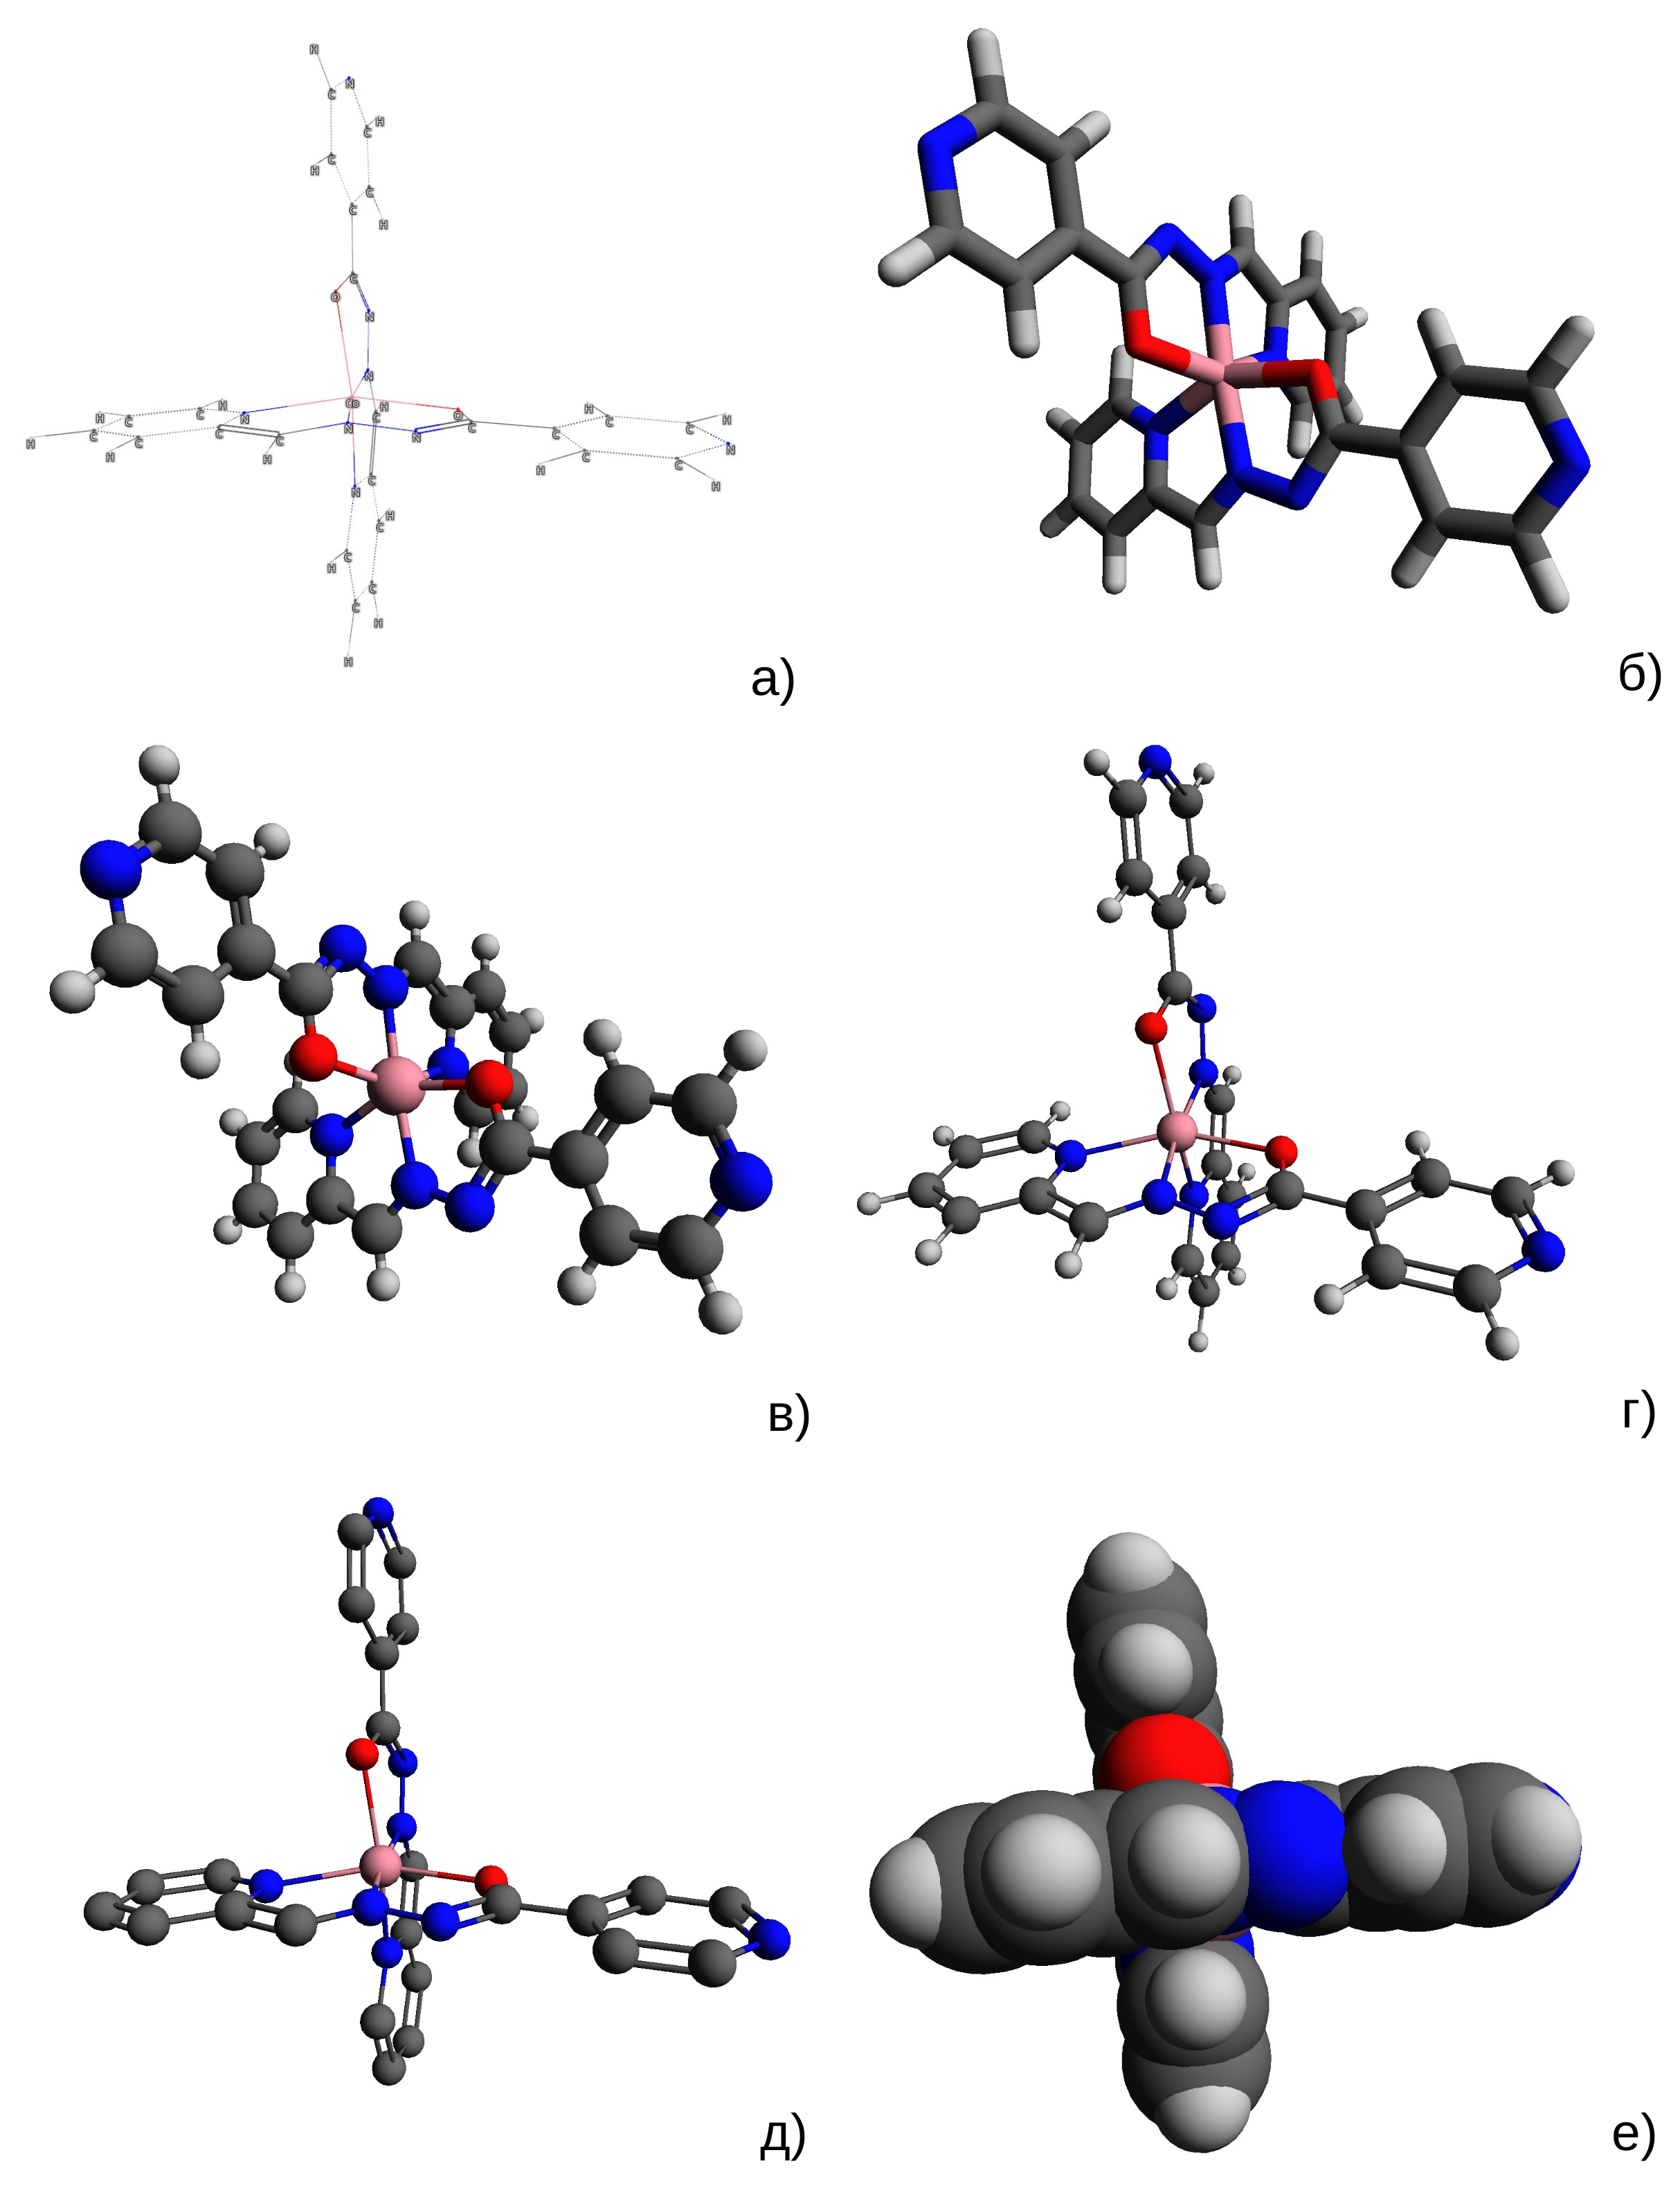
\includegraphics[width=8cm]{20_2016_Litvenenka3.png}
  \caption{Разные способы отображения 3D геометрии молекулы (оптимизированная путем квантовохимического моделирования геометрия комплексного соединения кобальта(II) с основанием Шиффа из 2-пиридилкарбальдегида и гидразида 4-пиридилкарбоновой кислоты, моделирование описано нами в работе ~\cite{Litvenenka2}): а) каркас; б) стержни; в) шары и стержни; г) шары и стержни с уменьшенными радиусами; д) шары и стержни с уменьшенными радиусами без атомов водорода; е) сферы ван дер Ваальса. Построено с использованием программы Avogadro.}
  \label{Litvenenka3}
\end{figure} 

Размеры изображений атомов и связей во всех моделях, кроме размеров сфер ван дер Ваальса, являются условными величинами, и их выбор определяется исключительно удобством представления "--- чем больше размеры, тем легче восприятие отдельных атомов, но тем больше атомы заслоняют друг друга. Для общего анализа геометрии сложной молекулы, состоящей из сотен атомов, больше подойдет изображение в виде каркаса, для подробного анализа более простых молекул "--- шаростержневая модель. Особое место занимает отображение атомов в виде сфер с радиусом, равным ван-дер-ваальсовским радиусам этих атомов, которое позволяет оценить пространство, доступное для других молекул.

В отличие от 2D-рисунков, использование меток и подписей в 3D-изображениях молекулярных структур ограничено, потому более интенсивно используются цветовые схемы (например, раскрашивание атомов разных элементов в разные цвета). Это ведет к получению более эффектных изображений, но усложняет подготовку рисунков для черно-белой печати.

Примеры свободных программ: Avogadro, Gabedit, PyMOL. В целом, наиболее известные и продвинутые 3D визуализаторы относятся к свободному ПО.

3D-визуализаторы, как правило, имеют инструменты для вращения, приближения-удаления, перемещения изображаемой молекулы, а также для измерения расстояний между атомами, углов между тройками атомов, а также диэдральных углов между плоскостями, задаваемыми четырьмя атомами.

В ситуациях, когда координаты атомов в некоторой молекуле из эксперимента неизвестны, и необходимо получить приближенное строение молекулы, для которой известно только химическое строение (связность атомов), важным функционалом 3D-визуализаторов является возможность <<рисования>> молекул и первичной оптимизации их геометрии (последняя, как правило, заключается поиске геометрии, имеющей минимальную энергию, методом молекулярной механики, в ряде случаев с применениями ограничений на изменения координат). Примером программы, реализующей такую возможность, является Avogadro, основанная на библиотеке OpenBabel (которая, среди других вариантов, реализует силовое поле UFF ~\cite{Litvenenka4}, параметризованное для всех элементов от водорода до лоуренсия, что позволяет <<рисование>> как органических, так и неорганических, в том числе металлокомплексных, молекул).

3D-визуализаторы используются также как средство для анализа результатов квантовохимического моделирования, в том числе построения изображений молекулярных орбиталей (рис. ~\ref{Litvenenka4}), форм нормальных колебаний (в виде векторов или в виде анимации), траекторий молекулярной динамики и т.д.

\begin{figure}[h!]
  \centering
  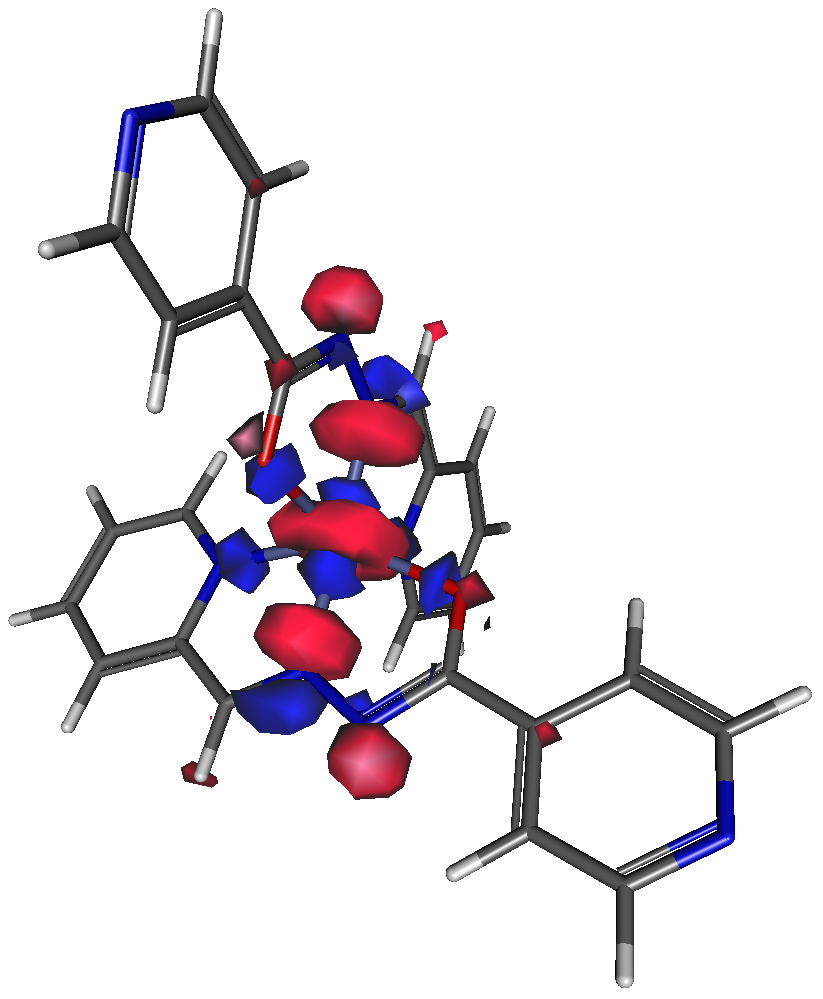
\includegraphics[width=5cm]{20_2016_Litvenenka4.png}
  \caption{75\% изоповерхность высшей занятой молекулярной орбитали ($\alpha$) комплексного соединения кобальта(II) с основанием Шиффа из 2-пиридилкарбальдегида и гидразида 4-пиридилкарбоновой кислоты (моделирование описано нами в работе ~\cite{Litvenenka3}), сгенерированная с помощью программы Gabedit.}
  \label{Litvenenka4}
\end{figure} 


Полученные изображения молекулярных структур сохраняются в специальных форматах (как правило, содержащих в том или ином виде координаты атомов и описание связей) и могут быть экспортированы в растровые или векторные изображения (в отличие от 2D-редакторов, возможности по добавлению текста или элементов схем в 3D редакторах намного беднее, однако, это можно сделать с помощью графических редакторов). Кроме того, ряд программ имеет возможность экспортировать сценарий для создания POV-Ray сцены (с ограниченными настройками, рис. ~\ref{Litvenenka5}).

\begin{figure}[h!]
  \centering
  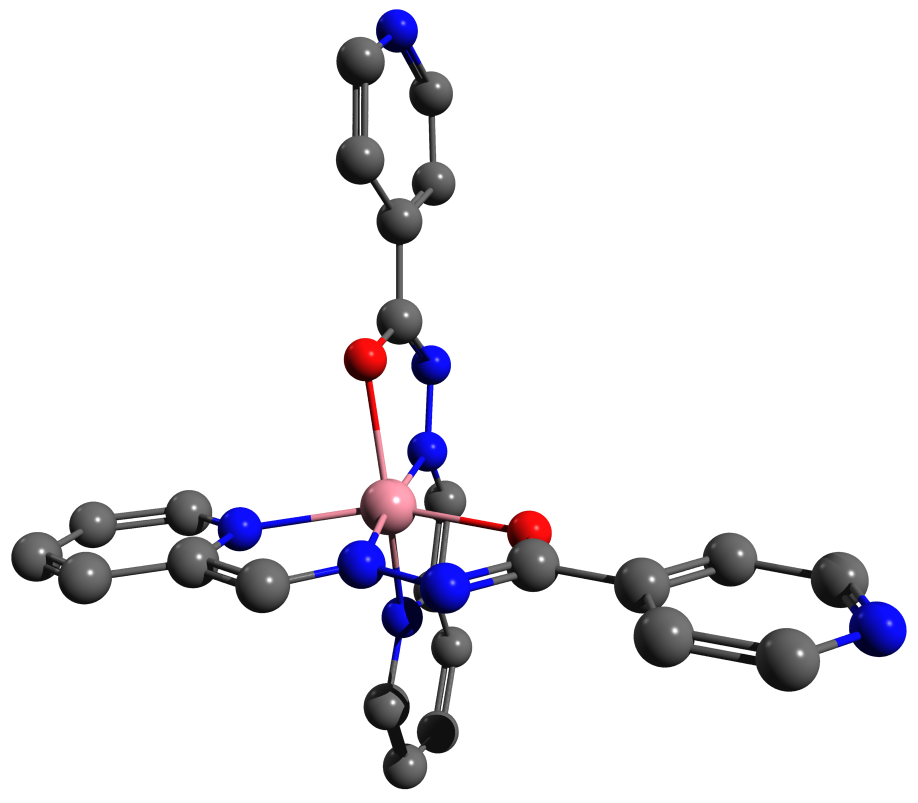
\includegraphics[width=5cm]{20_2016_Litvenenka5.png}
  \caption{3D геометрия молекулы (оптимизированная путем квантовохимического моделирования геометрия комплексного соединения кобальта(II) с основанием Шиффа из 2-пиридилкарбальдегида и гидразида 4-пиридилкарбоновой кислоты, моделирование описано нами в работе ~\cite{Litvenenka3}) в виде шаростержневой модели с уменьшенными радиусами без атомов водорода, сгенерированная с помощью POV-Ray, исходный файл для рендеринга создан программой Avogadro.}
  \label{Litvenenka5}
\end{figure} 
  
Существуют плагины, позволяющие работу с молекулами в \linebreak Blender, однако их функционал, равно как и размер импортируемых молекул, ограничены.

\subsubsection*{Визуализаторы кристаллических структур.}

Во многом похожи на 3D-визуализаторы, но отличаются полноценной возможностью работать с кристаллическими структурами "--- бесконечными периодическими системами (рис. ~\ref{Litvenenka6}). Соответственно, этот класс программ имеет возможность размножать элементы кристаллической решетки необходимое число раз операциями трансляции, ограничивать отображение отдельными цепочками или слоями с учетом трансляций, наращивать отображаемую структуру с учетом трансляций, ориентировать структуру вдоль осей элементарной ячейки и т.д. Дополнительными востребованными возможностями является анализ пористой структуры "--- объем (процент) пустот в кристалле, диаметр и форма пор, в том числе (в случае пор сложного строения) диаметр и форма сужений и расширений пор. Некоторые визуализаторы кристаллических структур (или сопряженные с ними программы) умеют также получать структуры путем обработки данных рентгеноструктурного анализа.

\begin{figure}[h!]
  \centering
  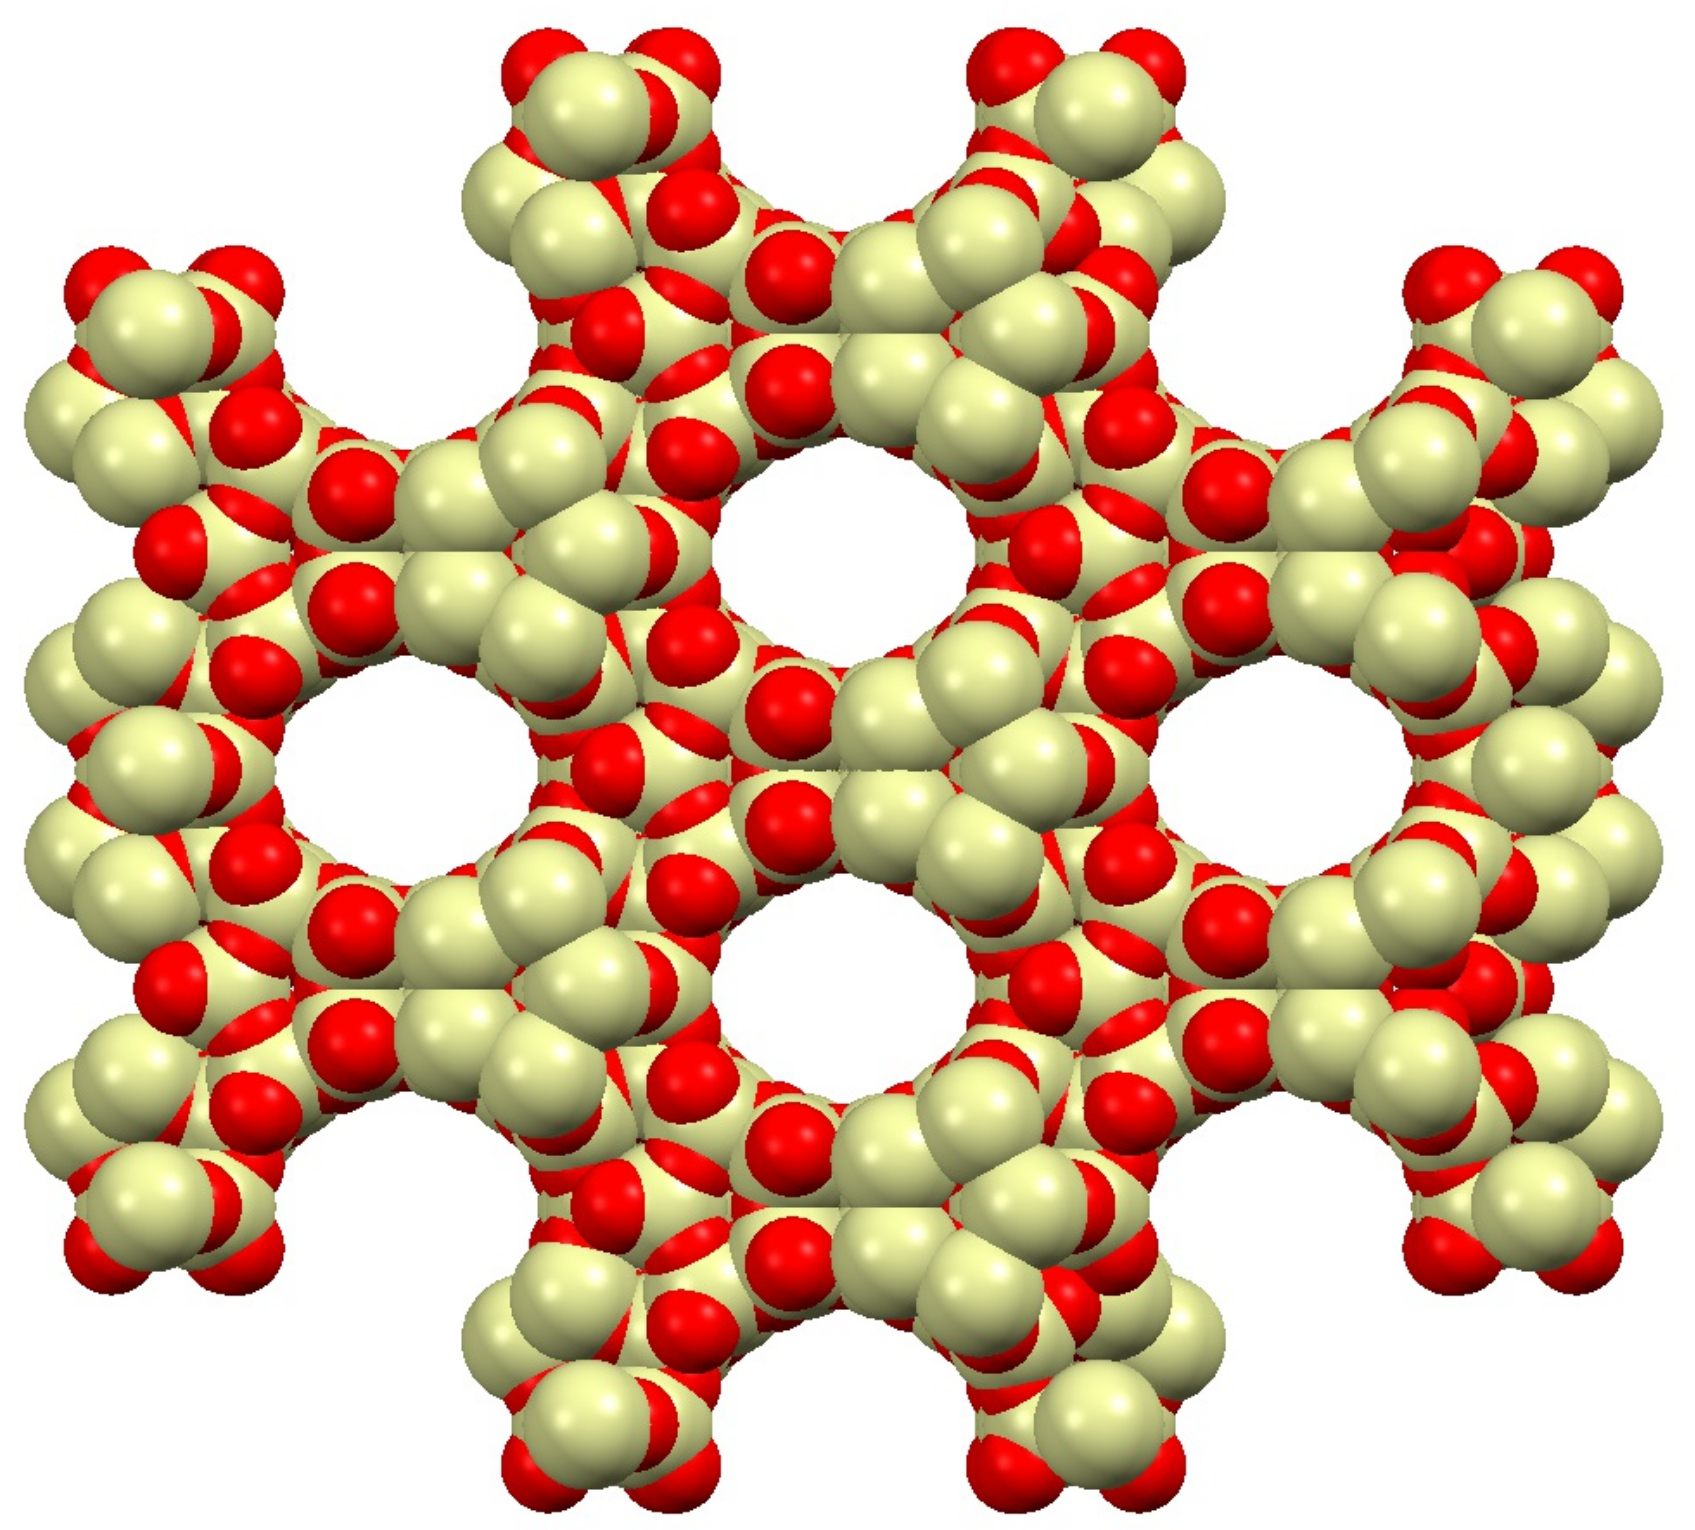
\includegraphics[width=5cm]{20_2016_Litvenenka6.png}
  \caption{Кристаллическая структура цеолита UTL, построенная в програме Mercury (proprietary freeware), модель "--- сферы ван дер Ваальса. На рисунке видны поры кристаллической структуры UTL.}
  \label{Litvenenka6}
\end{figure} 
К сожалению, в свободном ПО возможности работы с кристаллическими структурами крайне ограничены.

\subsubsection*{Текущие проблемы и задачи.}

\begin{itemize}
  \item Потребность в новых возможностях манипуляции кристаллическими структурами, в частности, подготовка входных данных и анализ результатов для квантовохимических расчетов с периодическими краевыми условиями (генерация суперячеек, преобразование в специфические форматы файлов, добавление гостевых молекул и т.д.);
  \item Продвинутый анализ микропористой (с диаметром пор до 2 нм) структуры: характеризация размеров и формы пор с учетом того, что размер поры сравним с размерами атомов (т.е. форма поры в значительной степени определяется расположением отдельных атомов);
  \item Поиск ответа на вопрос о возможности вхождения гостевой молекулы в микропору "--- геомерические критерии для сложных по форме пор и молекул, энергетические критерии (энергия активации диффузии молекулы в поре).
\end{itemize}

Для решения части этих задач нужен поиск или написание программного обеспечения, способного выполнять соответствующие \linebreak действия, тогда как для последней задачи необходима разработка новых теоретических подходов. Некоторые работы на уровне \emph{proof of concept} ведутся нами: так, доступность пор координационного полимера HKUST-1 (бензолтрикарбоксилата меди), катализирующего сочетание салицилового альдегида с нитрометаном с образованием \emph{транс}-нитровинилфенола, для реагентов и продукта реакции была показана нами путем определения величины энергии активации диффузии молекул в поре HKUST-1 методом молекулярной механики ~\cite{Litvenenka5}.

\subsubsection*{Выводы.}

Таким образом, программное обеспечение для визуализации химического строения вещества является важным инструментом в работе химика, применяемым для ряда связанных между собой задач: анализа строения вещества, подготовки и интерпретации результатов компьютерного моделирования химических веществ и процессов, а также подготовки материалов для публикаций. Свободное ПО такого типа развито недостаточно (за исключением 3D-визуализаторов молекулярных структур). Кроме того, в современной химии существуют задачи по анализу строения химических веществ, не решаемые или плохо решаемые с помощью существующих программ (в особенности свободных). Дальнейшее развитие визуализаторов химического строения вещества требует совместной работы специалистов в области химии и программирования и представляет собой важную задачу для развития современной химической науки.

\begin{thebibliography}{99}

\bibitem{Litvenenka1} S. H. Chanteau, J. M. Tour, <<Synthesis of Anthropomorphic Molecules:  The NanoPutians>>, \emph{J. Org. Chem.}, \textbf{2003}, 68(23):8750–8766.
\bibitem{Litvenenka2} A. Crum Brown, <<On the Theory of Isomeric Compounds>>, \emph{Transactions of the Royal Society of Edinburgh}, \textbf{1864}, 23:707–719.
\bibitem{Litvenenka3} A. S. Lytvynenko,   S. V. Kolotilov, M. A. Kiskin, I. L. Eremenko, V. M. Novotortsev, <<Modeling of catalytically active metal complex species and intermediates in reactions of organic halides electroreduction>>, \emph{Phys. Chem. Chem. Phys}, \textbf{2015}, 17:5594–5605
\bibitem{Litvenenka4} A. K. Rappe, C. J. Casewit, K. S. Colwell, W. A. Goddard III, W. M. Skiff, <<UFF, a full periodic table force field for molecular mechanics and molecular dynamics simulations>>, \emph{J. Am. Chem. Soc.}, \textbf{1992}, 114(25):10024–10035.
\bibitem{Litvenenka5} S. A. Sotnik, K. S. Gavrilenko, A. S. Lytvynenko, S. V. Kolotilov, <<Catalytic activity of copper(II) benzenetricarboxylate (HKUST-1) in reactions of aromatic aldehydes condensation with nitromethane: Kinetic and diffusion study>>, \emph{Inorg. Chim. Acta}, \textbf{2015}, 426:119–125.
\end{thebibliography}
\end{document}
